\section{Actividad No 02 – Reconociendo la estructura} 

\begin{enumerate}[1.]
	\item Se requiere determinar la estructura de la tabla DEPARTMENTS y sus datos.
	\\
	\\SP\_HELP 'DEPARTMENTS'

	\begin{center}
	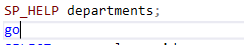
\includegraphics[width=9cm]{./Imagenes/actividad_02_01a} 
	\end{center}

	\begin{center}
	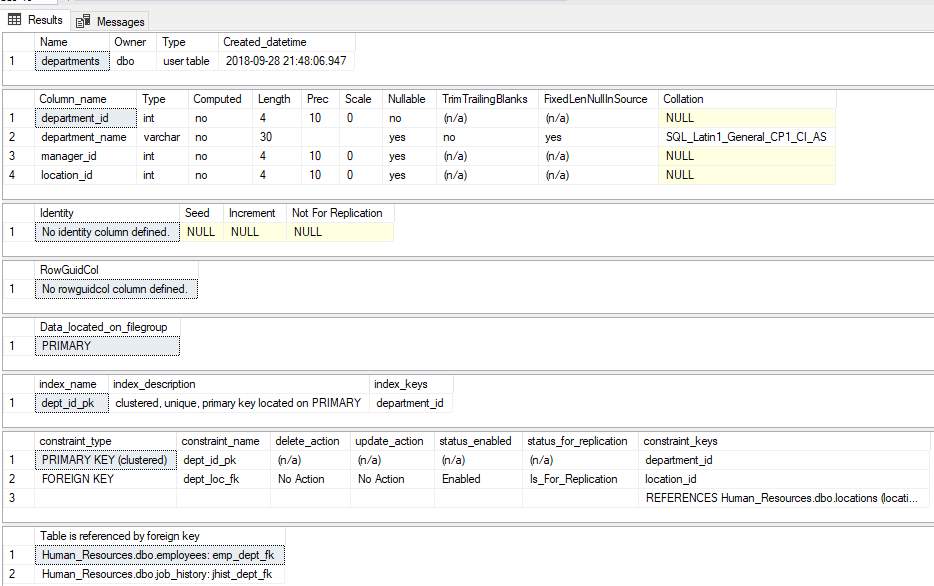
\includegraphics[width=15cm]{./Imagenes/actividad_02_01} 
	\end{center}

	\item El departamento de Recursos Humanos requiere un reporte que muestre los campos: employee\_id, last\_name y job\_id, asicomo el campo hire\_date con el alias StartDate.
	\\
	\\SELECT emp.employee\_id, \\
	emp.last\_name, \\
	emp.job\_id, \\
	emp.hire\_date AS StartDate \\
	FROM employees AS emp; 

	\begin{center}
	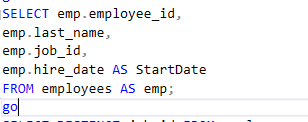
\includegraphics[width=10cm]{./Imagenes/actividad_02_02a} 
	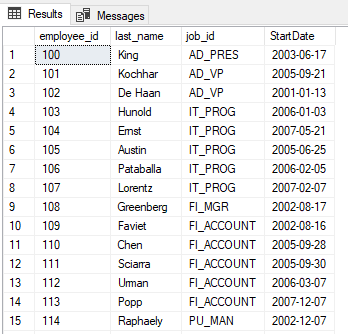
\includegraphics[width=10cm]{./Imagenes/actividad_02_02} 
	\end{center}

	\item Finalmente el departamento de Recursos Humanos requiere un listado de todos valores del campo JOB\_ID de la tabla EMPLOYEES pero que se muestren de forma única y no repetida.
	\\
	\\SELECT DISTINCT job\_id FROM employees; 

	\begin{center}
	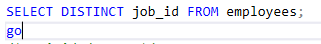
\includegraphics[width=11cm]{./Imagenes/actividad_02_03a} 
	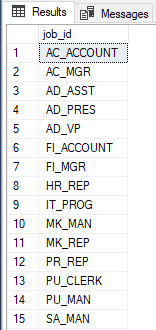
\includegraphics[width=6cm]{./Imagenes/actividad_02_03} 
	\end{center}

\end{enumerate}


